\documentclass{article}

\usepackage{lipsum}
\usepackage[margin=1.5in]{geometry}
\usepackage{titlesec}
\usepackage{graphicx}
\usepackage{amsmath}

\usepackage{mathtools, amssymb, nccmath}
\usepackage{bigstrut, changepage, lipsum}

\newcommand{\code}{\texttt}
\newcommand{\norm}[1]{\left\lVert#1\right\rVert}

\usepackage{siunitx} % Required for alignment


% Specify images directory
\graphicspath{ {./report-images/} }

% Header and Footer stuff
\usepackage{fancyhdr}
\pagestyle{fancy}
\fancyhead{}
\fancyfoot{}
\fancyfoot[R]{ \thepage\ }
\renewcommand{\headrulewidth}{0pt}
\renewcommand{\footrulewidth}{0pt}
\newcommand{\sectionbreak}{\clearpage}
\setlength{\parindent}{0pt}

%

\begin{document}

%----------------------------------------------------------------------------------------
%	TITLE PAGE
%----------------------------------------------------------------------------------------

\begin{titlepage} % Suppresses displaying the page number on the title page and the subsequent page counts as page 1
	\newcommand{\HRule}{\rule{\linewidth}{0.5mm}}% Defines a new command for horizontal lines, change thickness here
	
	\center % Centre everything on the page
	
	%------------------------------------------------
	%	Headings
	%------------------------------------------------
	
	\textsc{\Large Basic orthogonal and periodic functions}\\[0.5cm] % Major heading such as course name
	
	\textsc{\large Exercise 3}\\[0.5cm] % Minor heading such as course title
	
	%------------------------------------------------
	%	Title
	%------------------------------------------------
	
	\HRule\\[0.6cm]
	
	{\huge\bfseries Least-squares Approximation of Functions Using Orthogonal Polynomials}\\[0.25cm] % Title of your document
	
	\HRule\\[1.5cm]
	
	%------------------------------------------------
	%	Author(s)
	%------------------------------------------------
	
	\begin{minipage}{0.4\textwidth}
		\begin{flushleft}
			\large
			\textit{Author}\\
			\textsc{Cesare De Cal} % Your name
		\end{flushleft}
	\end{minipage}
	~
	\begin{minipage}{0.4\textwidth}
		\begin{flushright}
			\large
			\textit{Professor}\\
			\textsc{Annie Cuyt}\\ % Supervisor's name
			[0.25cm]
			\textit{Assistant Professor}\\
			\textsc{Ferre Knaepkens} % Supervisor's name

		\end{flushright}
	\end{minipage}
		
	\vfill\vfill\vfill
	
	{\large\today}
		
	\vfill
	
\end{titlepage}

%----------------------------------------------- Introduction ------------------------------------------------------
\section{Introduction}\label{sec:intro}
This exercise asks to compute the Chebyshev approximation
$$t(x)=\sum^n_{j=0}{a_jT_j(x)}$$

for the functions $f(x)=\cos(2x)$ and $f(x)=cos(4x)$ over the interval $[-\pi,\pi]$ for $n = 6$ and then plot the original functions with the approximations and draw conclusions on the results.


%---------------------------------- Tools ---------------------------------------------------------------------------
\section{Tools}
\section{Computation}
\section{Plot}
%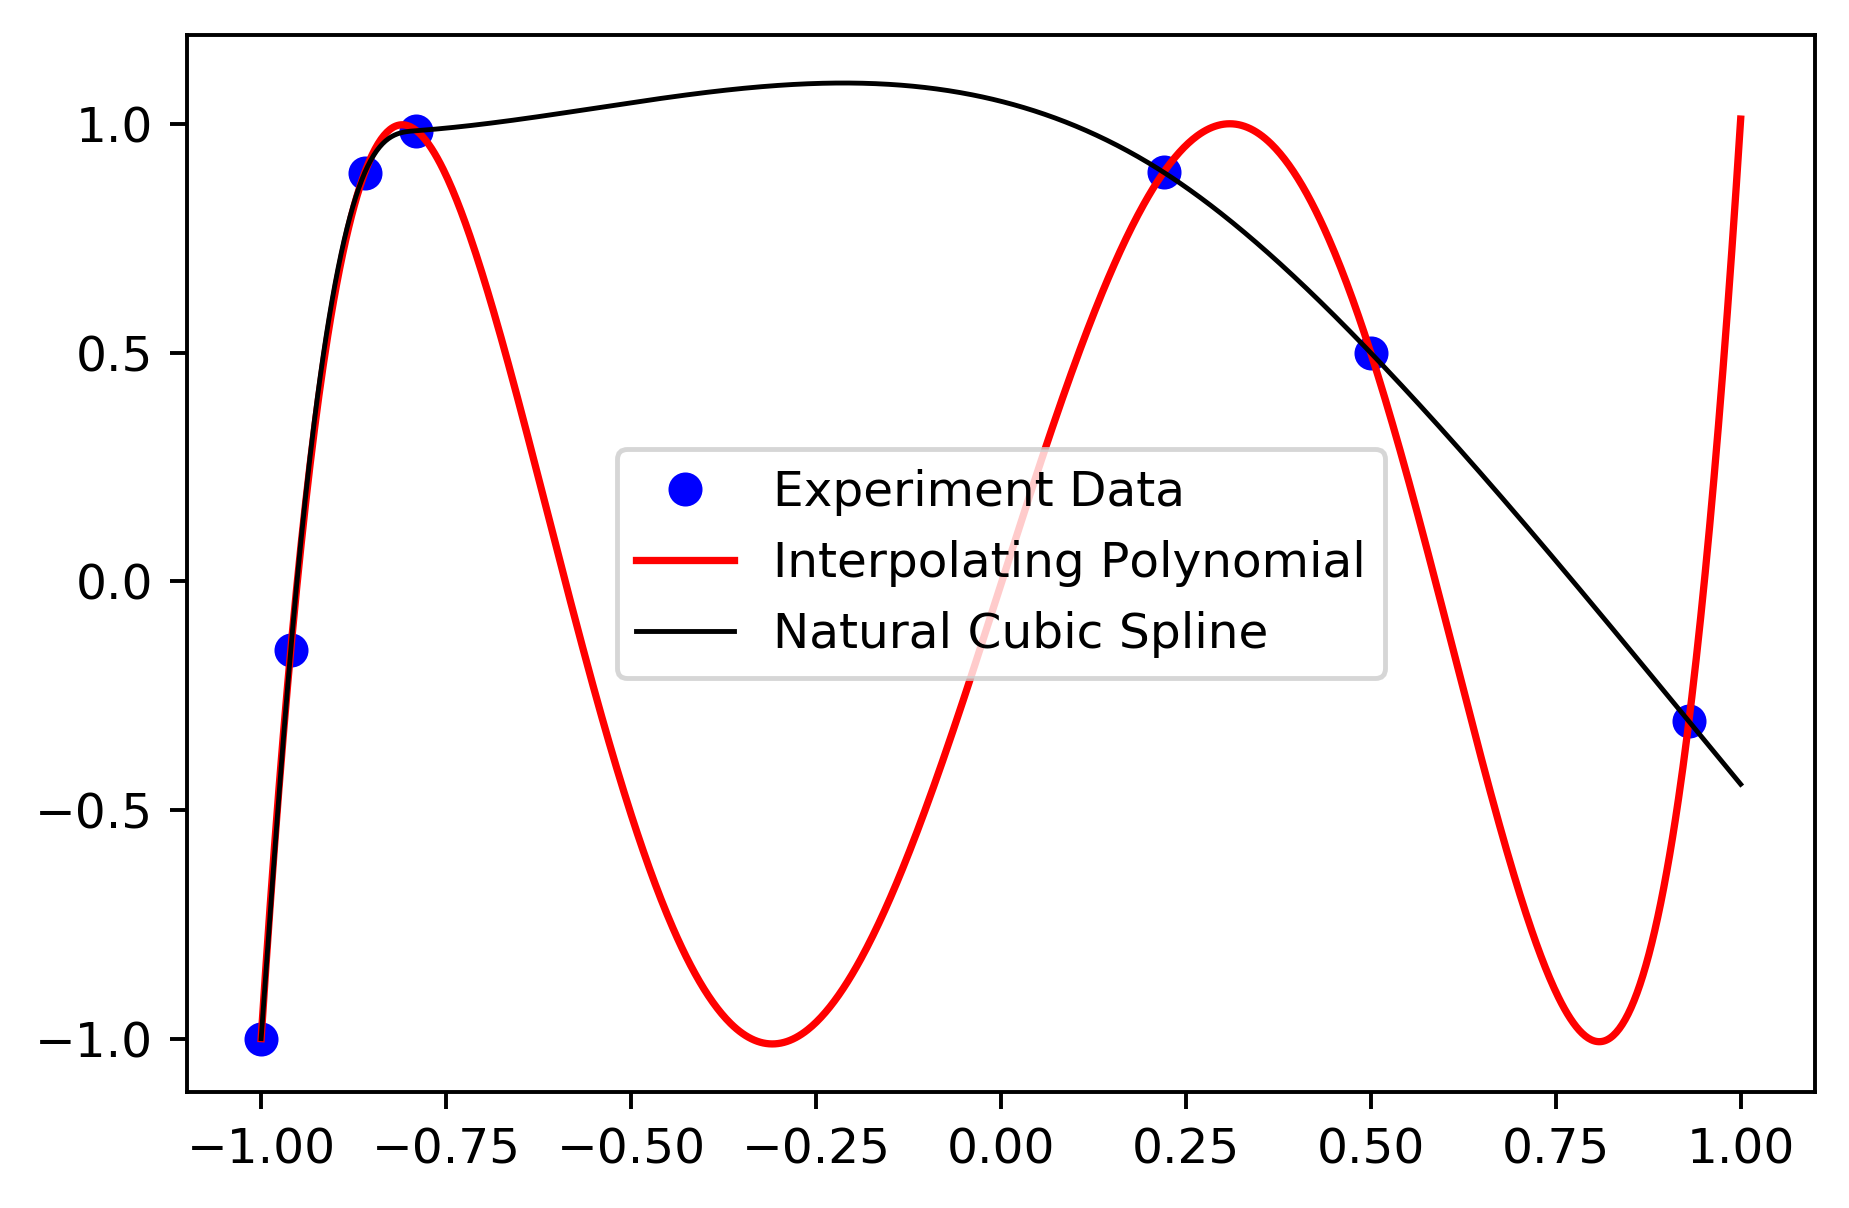
\includegraphics[width=\textwidth,height=\textheight,keepaspectratio]{graph.png}
\section{Observations}
\end{document}